% ---- Modele TP PC V2 -----------
\documentclass[a4paper,9pt,french]{scrartcl}
\usepackage[T1]{fontenc}%---pour l'encodage d'entr\'ee
\usepackage{array}%---pour les tableaux
\usepackage{titlesec}%---modification des titres
\usepackage{ulem}%---pour le soulignage
\usepackage[dvipsnames]{xcolor}%---pour avoir d'autres couleurs
\usepackage{color}%---pour avoir les couleurs de base
\usepackage{babel}%---pour les trucs de langue et la francisation

\usepackage{graphicx}%----pour mettre des images
\usepackage[utf8]{inputenc}%---encodage
\usepackage{geometry}%---pour modifier les tailles et mettre a4paper
%\usepackage{awesomebox}%---pour les boites d'exercices, de pbq et de croquis ---d\'esactiv\'e pour les TP de PC
\usepackage{tikz}%---pour dessiner + d\'ependance de chemfig
%\usepackage{tabularx}%---pour dimensionner automatiquement les tableaux avec variable X
\usepackage{fancyhdr}%---pour les en-t\^ete personnalis\'ees
\usepackage{blindtext}%---pour les liens
\usepackage{hyperref}%---pour les liens (\`a mettre en dernier)
\usepackage{caption}%---pour la francisation de la l\'egende table vers Tableau
 \usepackage{float}% --- pour placer les figures et tableaux où l'on souhaite avec argument H
 \usepackage{multicol}

\captionsetup{labelfont=sc}%---pour la francisation de la l\'egende table vers Tableau
\def\frenchtablename{Tableau}%---pour la francisation de la l\'egende table vers Tableau
\pagestyle{fancy}
\renewcommand\headrulewidth{1pt}
\fancyhead[L]{TP 5}
\fancyhead[R]{Saux Paulhenry}
\title{Compte rendu de TP 5}
\date{}
\author{}

\geometry{a4paper}
% ----------- Création des commandes de couleur ----------
\makeatletter
\newcommand{\coloruline}[2]{%
        \UL@protected\def\temp@uline{\leavevmode \bgroup
            \markoverwith{\textcolor{#1}{\rule[-0.5ex]{2pt}{0.4pt}}}%
        \ULon}%
        \temp@uline{#2}%
    }

    \newcommand{\coloruuline}[2]{%
        \UL@protected\def\temp@uuline{\leavevmode \bgroup
            \UL@setULdepth
            \ifx\UL@on\UL@onin \advance\ULdepth2.8\p@\fi
            \markoverwith{\textcolor{#1}{\lower\ULdepth\hbox
                {\kern-.03em\vbox{\hrule width.2em\kern1\p@\hrule}\kern-.03em}}}%
        \ULon}%
        \temp@uuline{#2}%
    }

\makeatother

\renewcommand{\thesection}{\arabic{section}}
\renewcommand{\thesubsection}{\arabic{subsection}}
\renewcommand{\thesubsubsection}{\arabic{subsubsection}}
\begin{document}
% ---------------- Modification des titres de niveau 1,2 et 3 --------------------
\titleformat
{\section} % command
%[display] % shape
{\Large} % format
{\coloruuline{red}{\thesection. }} % label
{0ex} % sep
{\coloruuline{red}} % before-code
[] % after-code

\titleformat
{\subsection} % command
%[display] % shape
{\Large} % format
{\coloruline{red}{\thesection.\thesubsection. }} % label
{0ex} % sep
{\coloruline{red}} % before-code
[] % after-code

\titleformat
{\subsubsection} % command
%[display] % shape
{\large} % format
{\coloruline{ForestGreen}{\thesection.\thesubsection.\thesubsubsection. }} % label
{0ex} % sep
{\coloruline{ForestGreen}} % before-code
[] % after-code

\titleformat
{\chapter} % command
%[display] % shape
{\large} % format
{\coloruline{NavyBlue}{\thechapter \:- }} % label
{0ex} % sep
{\coloruline{NavyBlue}} % before-code
[] % after-code


% ---------------- Début du corps du document ------------------------------------

\section{Introduction}
Ce TP se décompose en quatre parties :
\begin{enumerate}
 \item Analyse qualitative du champ magnétique d'un aimant et application aux aiguilles d'une boussole
 \item Mesure des caractéristiques d'une bobine de Helmotz
 \item Mesure du champ au centre de la bobine
 \item Création d'un champ magnétique continu avec 2 bobines de Helmotz
\end{enumerate}
\section{Protocole}
\subsection{Analyse qualitative du champ d'un aimant}
\subsubsection{Matériel}
\begin{multicols}{2}
\begin{itemize}
 \item Barreau aimanté
 \item Aiguille montée sur son support
 \item Un teslamètre à sonde Hall
\end{itemize}
\subsubsection{Description du montage expérimental}
Nous plaçons la sonde du teslamètre (1) à différents points particuliers choisis autour du barreau aimanté (2).
\columnbreak
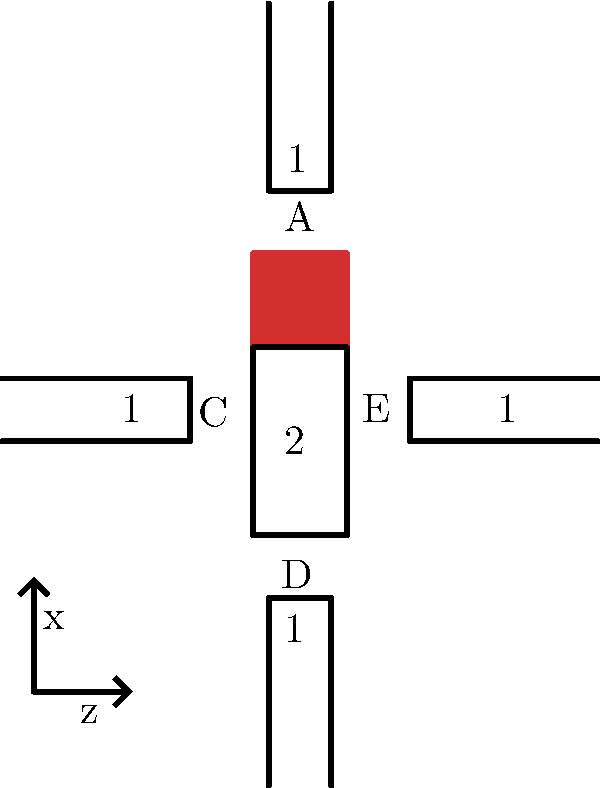
\includegraphics[scale=0.3]{aimants}
\end{multicols}
\subsubsection{Mesures à effectuer}
\begin{enumerate}
\item Étalloner la sonde de Hall
 \item Placer la sonde de Hall face à l'aimant, au premier point de mesure, à une distance de 1 cm.
 \item Relever la valeur Bx pour obtenir la valeur du champ dans la direction parallèle à la sonde
 \item Relever la valeur de Bz pour obtenir la valeur du champ dans la direction perpendiculaire à la sonde.
 \item En déduire les valeurs de Bx et Bz dans le repère lié à l'aimant.
 \item Répéter ces étapes pour les 3 autres points.
 \item Répéter ces étapes avec une distance de 2cm entre la sonde et le barreau
\end{enumerate}
\subsection{Mesure des caractéristiques d'une bobine de Helmotz}
\begin{multicols}{2}
\subsubsection{Matériel}
\begin{itemize}
 \item Bobine de Helmotz
 \item Règle graduée, cables électriques, support pour sonde de Hall
 \item Alimentation continue
 \item Un teslamètre à sonde Hall
\end{itemize}
\subsubsection{Description du montage expérimental}
Nous plaçons la sonde du teslamètre (1) sur le support fixe (5) afin que son extrémité se trouve au centre de la bobine (2). Nous déplaçons la bobine en la faisant glisser sur son support et nous relevons la distance de déplacement avec la règle graduée (4). La bobine est branchée à l'alimentation continue (3).
\end{multicols}
\begin{center}
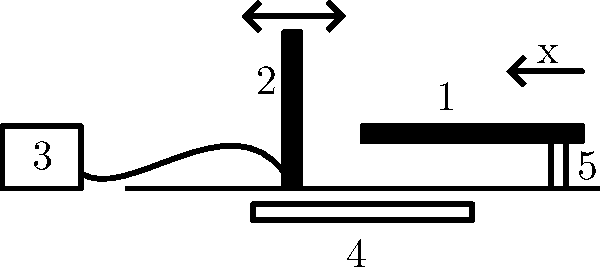
\includegraphics[scale=0.5]{bobine}
\end{center}
\subsubsection{Protocole}
\begin{enumerate}
\item Étalloner la sonde de Hall
 \item Placer la sonde de Hall dans son support de façon à ce que son extrémité se trouve à environ 10 cm (graduation de la règle). La précision de la position de l'extrmité n'est pas critique.
 \item Paramétrer l'alimentation continue à 1.5 A.
 \item Placer la bobine à 10 cm.
 \item Relever la valeur de Bx sur le teslamètre.
 \item Translater la bobine de \(\pm 1cm\).
 \item Relever la nouvelle valeur de Bx
 \item Répter les deux étapes précédentes pour obtenir une dizaine de valeur.
\end{enumerate}
\subsection{Mesure du champ au centre de la bobine}
\subsubsection{Matériel \& Description du montage expérimental}
Le matériel utilisé et le montage expérimental sont les m\^emes que dans la partie précédente, à l'ajout d'un ampèremétre près.
\subsubsection{Protocole}
\begin{itemize}
 \item Étalloner la sonde de Hall
 \item Placer la sonde au centre de la bobine (si la sonde n'a pas bougé, on peut se servir de la valeur de \(x_0\) trouvée en partie précédente pour placer présicément la sonde.)
 \item Régler l'intensité sur 0.5 A
 \item Mesurer \(B_x\)
 \item Répéter ces 2 étapes pour les autres valeurs de I
\end{itemize}
\subsection{Création d'un champ magnétique continu avec 2 bobines de Helmotz}
\subsubsection{Matériel \& Description du montage expérimental}
Le matériel utilisé et le montage expérimental sont les m\^emes que dans la partie précédente, à l'ajout d'une deuxième bobine, mobile, près.
\subsubsection{Protocole}
\begin{itemize}
 \item Étalloner la sonde de Hall
 \item Placer la sonde au centre des 2 bobines.
 \item Tracer sur la sonde une marque au niveau de la vis de maintient
 \item Tracer sur la sonde les graduations correspondants au distances pour lesquelles on souhaite mesurer une valeur de champ, en prenant comme origine la marque précédente.
 \item Replacer la sonde dans le support au niveau de la graudation 0.
 \item Mesurer la valeur du champ
 \item Répéter ces 2 étapes pour chaque graduation.
\end{itemize}

\section{Mesures}
\subsection{Analyse qualitative d'un aimant}
\subsubsection{Données}
\begin{center}
\begin{tabular}{llll}
Point & Distance d (cm) & Valeur de champ Bx (mT) & Valeur de champ Bz (mT)\\
A & 1.0 & 4.0 & 0.25\\
A & 2.0 & 2.2 & 0.1\\
E & 1.0 & -2.9 & 1.0\\
E & 2.0 & -1.7 & 0.5\\
C & 1.0 & -2.7 & -1.0\\
C & 2.0 & -1.4 & -0.5\\
D & 1.0 & 4.2 & 0.9\\
D & 2.0 & 2.1 &0.0
\end{tabular}
\end{center}
\subsubsection{Incertitude}
Les incertitudes concernent la mesure de la distance entre le barreau et la sonde et la mesure du champ. Ces dernières sont toutes les 2 de type B. Pour la mesure de la distance, l'incertitude est lié à la graduation de la règle utilisée, ici d'une précision au dixième de cm. Celle sur la mesure du champ est liée à la précion du teslamètre, au maximum de 0.01 mT. On a donc : \[u(d) = \frac{0.1}{\sqrt{3}}cm\] et  \[u(Bx) = u(Bz) = \frac{0.01}{\sqrt{3}}mT\]
\subsection{Mesure des caractéristiques d'une bobine de Helmotz}
\begin{multicols}{2}
\subsubsection{Données}
\begin{center}
\begin{tabular}{ll}
Distance (cm) & Bx (mT)\\
-5.0 & 0.40\\
-4.0 & 0.53\\
-3.0 & 0.68\\
-2.0 & 0.85\\
-1.0 & 1.06\\
0.0 & 1.22\\
1.0 & 1.36\\
2.0 & 1.40\\
3.0 & 1.31\\
4.0 & 1.17\\
5.0 & 0.99\\
6.0 & 0.80\\
7.0 & 0.63\\
8.0 & 0.49\\
9.0 & 0.38\\
10.0 & 0.27
\end{tabular}
\end{center}
\subsubsection{Incertitude}
La mesure de distance et de champ magnétique ont une incertitude de type B. De la m\^eme façon que dans la partie précédente, l'incertitude liée à la mesure de la distance est de\footnote{L'incertitude liée à la position de l'extrémité de la sonde n'a pas d'importance ici, car le potentiel décalage sera pris en compte dans notre modélisation. On ne va donc pas ajouter d'incertitude systématique lié au décalage entre le centre de la bobine et la position de l'extrémité de la sonde.} \[u(d) = \frac{0.1}{\sqrt{3}}cm\]
L'incertitude liée à la meure du champ est, comme dans la partie précédente \[u(Bx) = u(Bz) = \frac{0.01}{\sqrt{3}}mT\]
\end{multicols}
\subsection{Mesure du champ au centre de la bobine}
\subsubsection{Données}
\begin{multicols}{2}
\begin{center}
\begin{tabular}{ll}
Intensité (A) & Champ Bx (mT)\\
0.50 & 0.48\\
1,00 & 0.99\\
1.25 & 1.20\\
1.50 & 1.43\\
1.75 & 1.69\\
2.00 & 1.92
\end{tabular}
\end{center}

\subsubsection{Incertitude}
Nous avons une incertitude sur la position de la sonde par rapport à la bobine, une incertitude sur l'intensité du courant et une sur le champ magnétique, toutes de type B. Celle sur l'intensité est liée à la précision de l'ampèremétre : \[u(I) = \frac{0.1}{\sqrt{3}}\] %TODO Precision
et celle sur le champ magnétique est toujours la m\^eme : \[u(Bx) = \frac{0.01}{\sqrt{3}}mT\]
\end{multicols}
L'incertitude la plus importante est celle sur la position de la sonde. En effet, bien que la graduation nous servant pour la placer a une précision de l'ordre du mm, il est difficile de savoir exactement où se trouve l'origine de la sonde. On estime donc cette incertitude à 1.5 cm, largeur du bout de la sonde. C'est l'incertitude qui domine cette manipulation, on peut négliger les autres. Ainsi, pour cette série de mesure, on suppose que \(x\in[-0.75, 0.75]\)cm ou \(x = (0\pm 0.75)\cdot 10^{-2}\)m.
\subsection{Création d'un champ magnétique continu avec 2 bobines de Helmotz}
\subsubsection{Données}
Nous avons choisie de faire les mesures pour des intensités de 1, 1.5 et 2 A\footnote{Nous avons choisie de ne pas faire les mesures pour I = 1 A pour les distances 2R et pour les bobines collées par manque de temps. Pour avoir l'incertitude la plus faible, nous avons gardé les 2 valeurs de I les plus élevées.} avec des distances dépendant du rayon de la bobine : \(\pm R, \pm \frac{R}{2}, \pm \frac{R}{4}\) avec un rayon mesuré à 6.75 cm.

\begin{figure}[H]
\begin{center}
\begin{tabular}{llllllll}
I (A)  \textbackslash d (cm) & 0 & 1.7 & -1.7 & 3.4 & -3.4 & 6.8 & -6.8\\
1.00&1.30 & 1.30 & 1.30 & 1.25 & 1.25 & 0.77 & 0.79 \\
1.50&1.97 & 1.97 & 1.98 & 1.91 & 1.87 & 1.15 & 1.19 \\
2.00&2.61 & 2.61 & 2.62 & 2.55 & 2.50 & 1.54 & 1.60
\end{tabular}
\end{center}
\caption{Données pour une distance entre les bobines de \(D = R\)}
\end{figure}

\begin{figure}[H]
\begin{center}
\begin{tabular}{llllllllll}
I (A)  \textbackslash d (cm) & 0 & 1.7 & -1.7 & 3.4 & -3.4 & 6.8 & -6.8 &10.3&-10.3\\
1.50&0.91 & 1.00 & 1.00 & 1.19 & 1.21 & 1.54 & 1.59&0.94&0.99 \\
2.00&1.23 & 1.33 & 1.34 & 1.57 & 1.62 & 2.06 & 2.01 &1.28&1.31
\end{tabular}
\end{center}
\caption{Données pour une distance entre les bobines de \(D = 2R\) avec des intensités de 1.5 et 2 A}
\end{figure}

\begin{figure}[H]
\begin{center}
\begin{tabular}{llllllll}
I (A)  \textbackslash d (cm) & 0 & 1.7 & -1.7 & 3.4 & -3.4 & 5.5 & -5.5\\
1.50&2.44 & 2.26 & 2.26 & 1.95 & 1.95 & 1.35 & 1.36 \\
2.00&3.26 & 3.01 & 3.04 & 2.64 & 2.62 & 1.81 & 1.82
\end{tabular}
\end{center}
\caption{Données pour une distance entre les 2 bobines collées avec des intensités de 1.5 et 2 A}
\end{figure}

\subsubsection{Incertitude}
Nous avons comme dans les parties précédentes une incertitude sur I et \(B_x\) liées à la précision des appareils de mesure. L'incertitude liée à la distance entre les bobines est aussi de l'ordre du mm. Ces dernières sont négligeables devant l'incertitude liée à la position de la sonde de Hall. Comme expliqué en 3.3.2, la méconnaissance de l'emplacement précis de l'origine de la sonde crée une incertitude systématique de \(\pm 0.75\)cm environ. Cette incertitude est grande devant celle liée à la graduation effectuée sur la règle. Cependant, nous nous servons de la vis du support pour positionner la graduation effectuée. Cette vis un diamètre de 5mm\footnote{L'incertitude obtenue avec cette méthode est bien plus petite qu'en mesurer directement la distance avec la règle fournie. C'est pourquoi nous avons utilisé cette méthode.}, on peut donc rauisonnablement ajouter une incertitude \(\pm 2\)mm sur les décalages succissifs de la sonde. L'incertitude finale liée à la distance de la sonde est donc de \[u(d) = \pm 1 cm\]
\section{Graphiques}
%TODO schema avec les lignes de champ.
\subsection{Mesure des caractéristiques d'une bobine de Helmotz et Mesure du champ au centre de la bobine}
\begin{figure}[H]
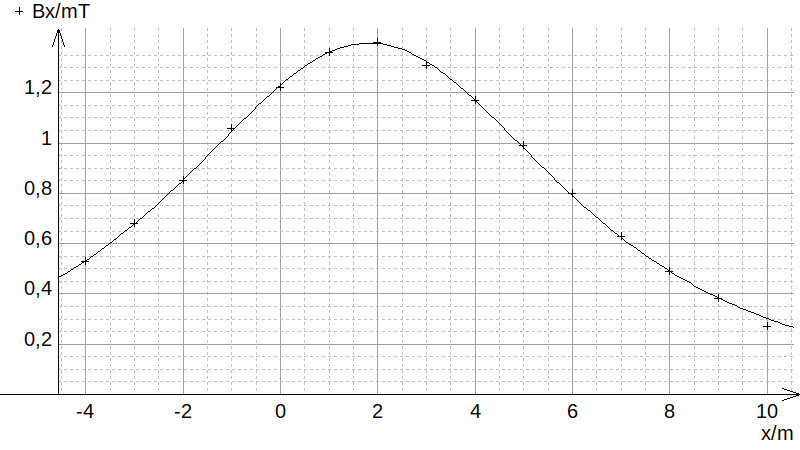
\includegraphics[scale=0.25]{part1}
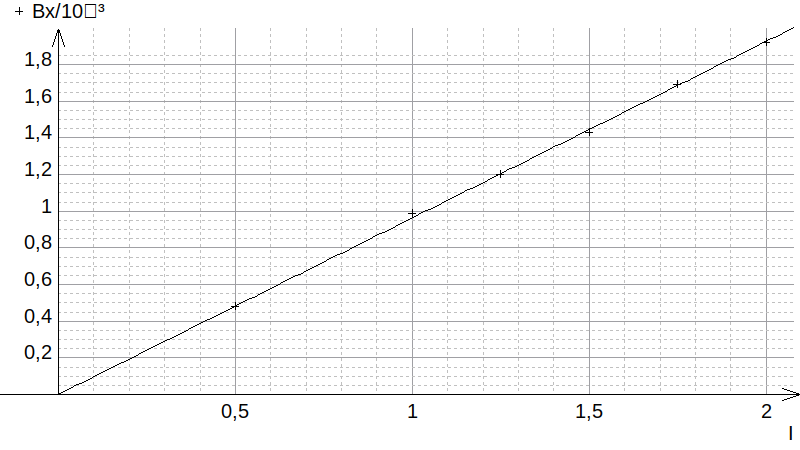
\includegraphics[scale=0.25]{part2}
\caption{Évolution du champ magnétique en fonction de la distance à la bobine puis en fonction de l'intensité.
Les ordonnées sont en mT et les abscices en cm pour le premier graphique et en A pour le deuxième.}
\end{figure}
\subsection{Création d'un champ magnétique continu avec 2 bobines de Helmotz}
\begin{figure}[H]
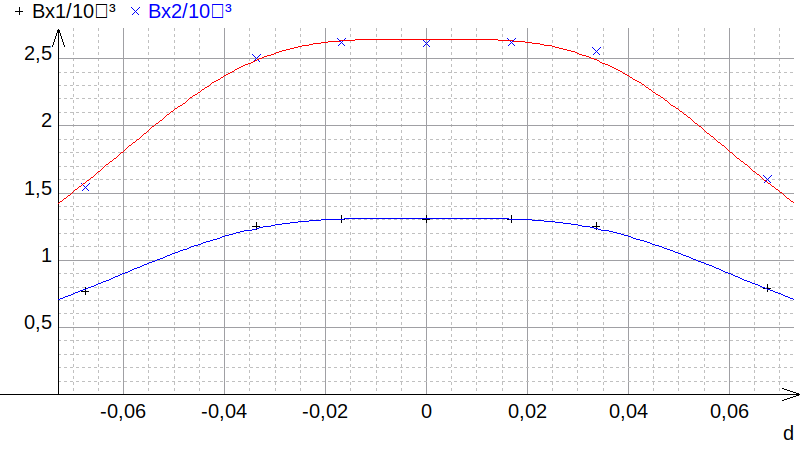
\includegraphics[scale=0.25]{part3}
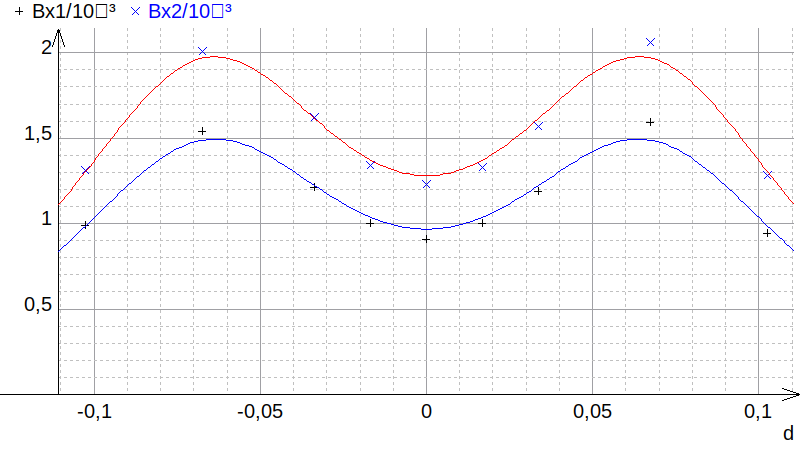
\includegraphics[scale=0.25]{part4}

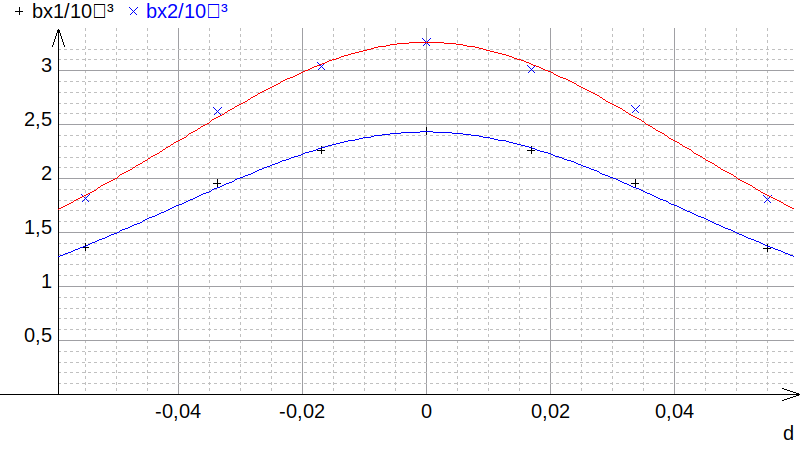
\includegraphics[scale=0.25]{part5}
\caption{Évolution du champ magnétique en fonction de la distance à la bobine et en fonction de l'intensité (1.5A en bleu et 2A en rouge). On représente les cas \(D = R, D = 2R, D\simeq 0\).
Les ordonnées sont en mT et les abscices en m.}
\end{figure}
\section{Exploitation des résultats}
\subsection{Analyse qualitative d'un aimant}

On retrouve bien le spectre de champ d'un aimant. De plus, comme l'aiguille rouge de la boussole est attirée par le pole - de l'aimant, on en déduit que le pole nord magnétique (le +) se trouve au sud et que le pole sud magnéique se trouve au nord !
\subsection{Mesure des caractéristiques d'une bobine de Helmotz}
\subsubsection{Détermination du rayon}
On peut modéliser la courbe obtenue par \begin{equation}B_x = A\frac{R^2}{(R^2+(x-x_0)^2)^{3/2}}\label{eq1}\end{equation} avec \(A, R, x_0\) à déterminer. Ici, \(x_0\) correspond en fait au décalage entre la position de l'origine de notre repère (normalement au centre de la bobine) avec le vrai centre de la bobine. C'est pour cette valeur de x que le champ est maximal. Plus x est petit, plus le positionnement expérimental de l'origine est proche de la position théorique.
On obtient \(A = (8.55\pm 0.047)\cdot 10^{-5} S.I, R = (6.13\pm0.05) cm, x_0=(1.83\pm0.02)cm S.I\). Le rayon trouvé est proche de la valeur mesurée expérimentalement avec la règle graduée, qui est de \((R_2 = 6.8\pm 0.5)cm\). L'incertitude sur cette valeur est liée à l'épaisseeur de la bobine et à la difficulté de mesurer précisément le diamètre des fils de bobine et non le support en lui-m\^eme.
\subsubsection{Vérification du résultat}
On peut calculer \(B_x\) avec
\begin{equation}
 B_x = \mu_0\frac{NI}{2}\frac{R^2}{(R^2+x^2)^{3/2}}
 \label{eq2}
\end{equation}
Par identification, avec \ref{eq1}, on a \[N = \frac{2A}{\mu_0I}\] On peut donc déterminer N. Avec les valeurs trouvées et donnéees fournies, on trouve \(N = 90,7\).

Avec la formule de propagationd des incertitudes, ici sur I et sur A, on obtient \[\frac{u(N)}{N} = \sqrt{ \left( \frac{u(A)}{A} \right)^2 + \left( \frac{u(I)}{I} \right)^2 }\]
En prenant \(u(I) = \frac{0.1}{\sqrt{3}}\)A et \(u(A) = 0.45\cdot10^{-6}\) SI, on obtient \[N = 91\pm3.5\] ce qui est cohérent avec les indications du fabricant (95 spires).
\subsection{Mesure du champ au centre de la bobine}
Comme au centre de la bobine, \(x=0\), avec \ref{eq2}, on a \[B_x = \mu_0 \frac{NI}{2}\frac{1}{R} = A I\] avec \(A = \frac{\mu_0N}{2R}\).

Les incertitudes sur R sont uniquement liées à celles sur A. Par la propagtion des incertitudes, on obtient que \(u(R) = R\frac{u(A)}{A}\).

On trouve \(A = (962.7\pm4.1)\cdot 10^{-6}\) SI puis \(R = (6.200\pm0.026)\cdot10^{-2}m\)
\subsection{Création d'un champ magnétique continu avec 2 bobines de Helmotz}
Dans cette situation, on trouve que \begin{equation}B(x)=\frac{\mu_0 N I}{2}\,R^2\left[ \frac{1}{\left(R^2+\left(x+\frac{d}{2}\right)^2\right)^{3/2}} +\frac{1}{\left(R^2+\left(x-\frac{d}{2}\right)^2\right)^{3/2}} \right]\end{equation} au point M d'abscice x. On peut modéliser les valeurs obtenues dans les cas \(d = R, 2R, 0\) en remplaçant la valeur de $d$ dans cette équation. Pour modéliser le cas ou \(d=0\), comme il n'est pas possible en pratique d'obtenir de telle conditions, on peut modéliser les bobines comme une seule spire de largeur infiniment petite. On aura alors une distance \(d=4.5\pm 0.2\) cm. L'incertide est liée au fait qu'expérimentalement, m\^eme si les supports des bobines sont collées, ces dernières ne le sont pas complètement car déformées.
\subsubsection{Cas d=R}
On remarque un plateau centré en l'origine. Sur 5 cm environ, le champ magnétique présente des valeurs semblables et peut \^etre qualifié d'uniforme (plateau de Helmotz). Cette configuration est donc utilisée pour obtenir des conditions expérimentales ou le champ doit \^etre uniforme le long d'un axe.
\subsubsection{Cas d=2R}
La distance est trop grande pour que les 2 bobines puissent intéragir efficacement pour produire le plateau de Helmotz. On obtient donc des valeurs pour un champ produit par 2 bobines distinctes, avec 2 maximas disnticts.
\subsubsection{cas d=0}
Bien que la distance ne soit pas nulle, les valeurs obtenues peuvent \^etre modélisées comme provenant d'une bobine de \(2\times N\) spires. Les 2 bobines se confondent alors en une seule.
\section{Conclusion}
Ce TP a permis d'étudier les champs magnétiques générés par un aimant puis par deux bobines.

Nous avons d'abord mené une analyse qualitative du champ d'un aimant, confirmant la structure dipolaire des lignes de champ.

L'étude d'une bobine de Helmholtz nous a permis de déterminer certaines de ses propriétés.

En analysant la variation du champ $B_x$ le long de l'axe de la bobine (Partie 4.2), nous avons déterminé son rayon $R$ par modélisation. La valeur obtenue est en accord avec la celle obtenue par la mesure du champ au centre. Nous avons pu en déduire le nombre de spires, $N = 91 \pm 3.5$, ce qui est cohérent avec les données constructeur (95 spires).

Enfin, le champ champ généré par deux bobines a été étudiée pour différentes distances $D$.

La configuration $D=R$ permet ainsi de créer un champ magnétique uniforme sur une zone centrale significative (un plateau de $\approx 5$ cm), ce qui peut \^etre utile pour de nombreuses expériences physiques.

% Les configurations $D=2R$ et $D \simeq 0$ ont mis en évidence la nécessité d'un espacement précis pour obtenir l'uniformité souhaitée. Lorsque $D=2R$, les deux maxima de champ restent séparés, tandis que pour $D \simeq 0$ (bobines "collées"), le dispositif se comporte comme une seule bobine de $2N$ spires.

Les incertitudes ont montré que la position précise de l'origine de la sonde de Hall était le facteur limitant le plus important dans nos manipulations. Il faudrait donc trouver un moyen de rendre ces mesures plus précises, en indiquant sur le bout de la sonde où se trouve précisement l'origine du capteur, puis en positionnant la sonde sur un rail afin de la déplacer selon un seul axe de façon plus précise.

\end{document}
